\begin{figure*}[p]
\centering
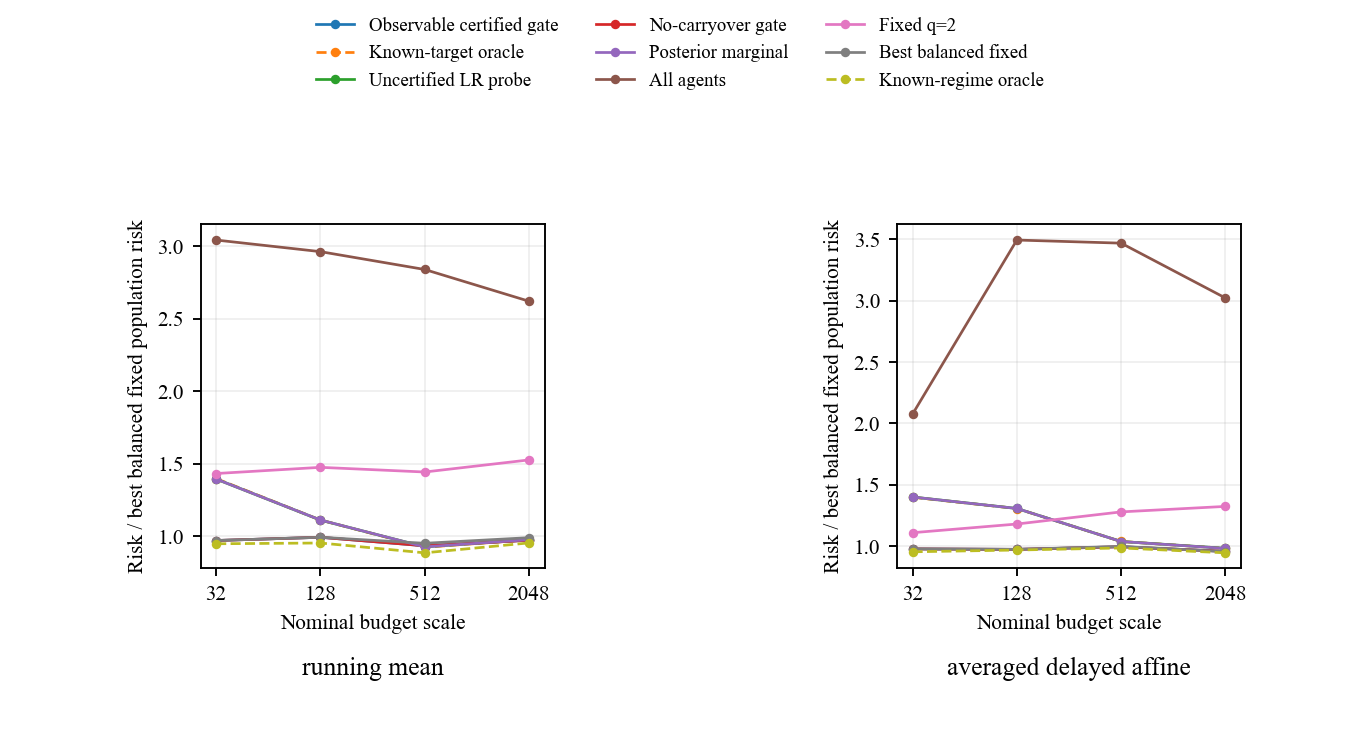
\includegraphics[width=\textwidth]{figures/observable_budget_20261021.png}
\caption{Observable study, all nine policies against budget scale. The native legend's known-target oracle is an evaluation-only centered-pilot reference, not a universal optimum; coincident curves are retained without offsets.}
\label{fig:observable-budget}
\par\medskip
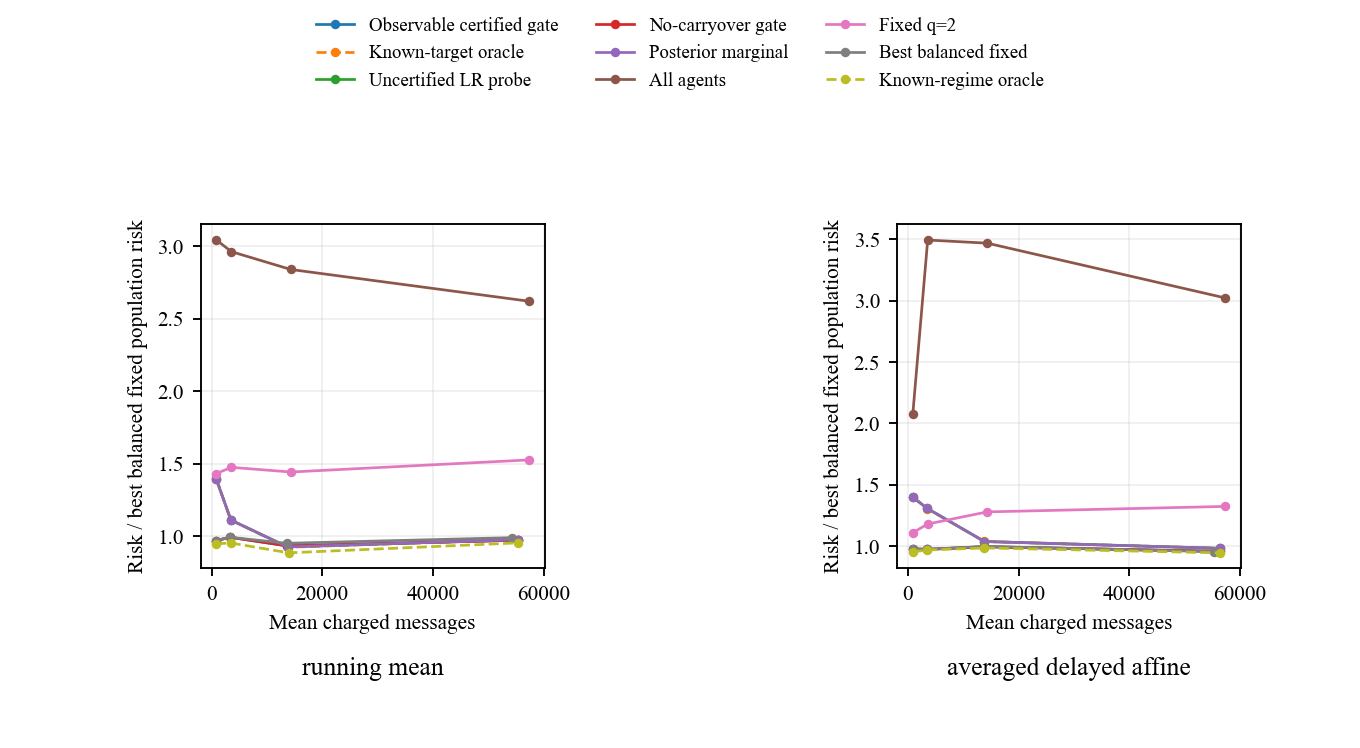
\includegraphics[width=\textwidth]{figures/observable_messages_20261021.png}
\caption{All observable-study policies against actual paid messages. Points connect distinct budget experiments rather than a common-resource stopping comparison.}
\label{fig:observable-messages}
\end{figure*}
\begin{figure*}[p]
\centering
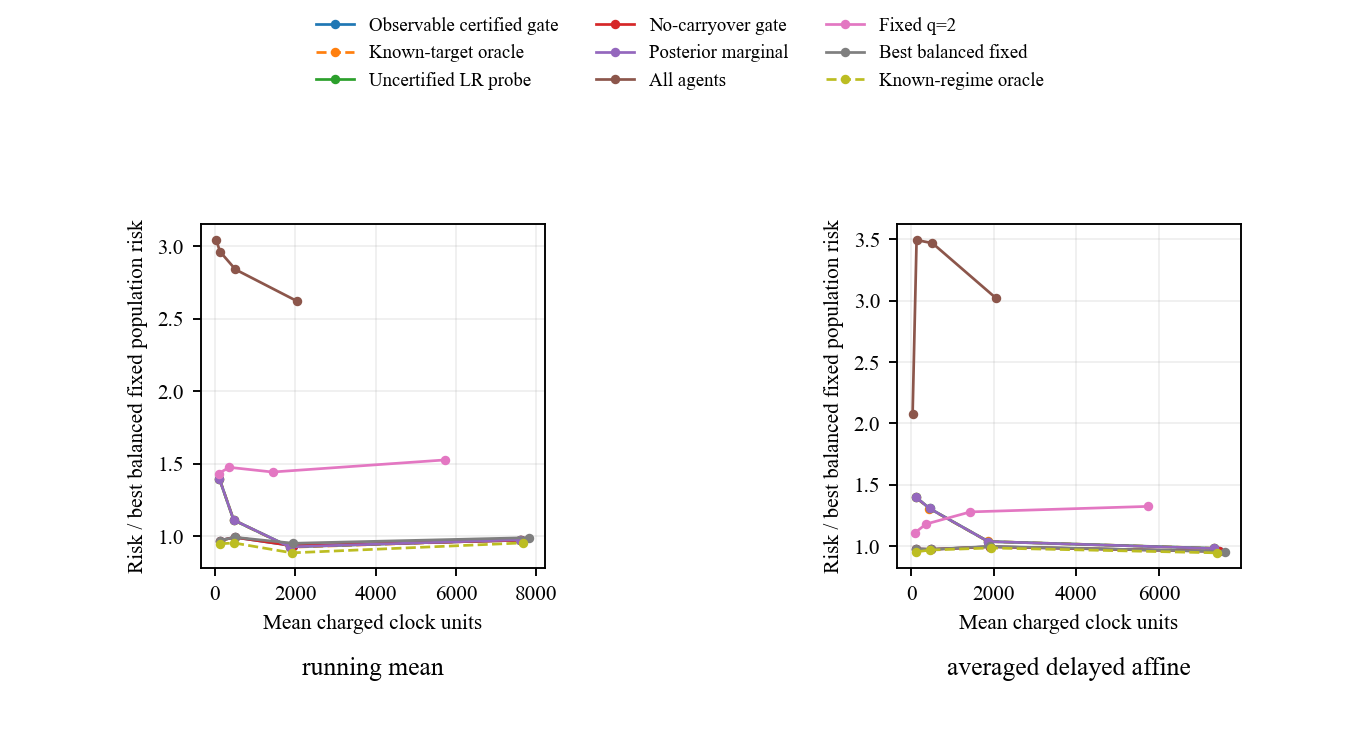
\includegraphics[width=\textwidth]{figures/observable_clock_20261021.png}
\caption{All observable-study policies against paid clock units; the fixed-prefix backstop and nine adverse fixed-comparison design means remain in the analysis.}
\label{fig:observable-clock}
\par\medskip
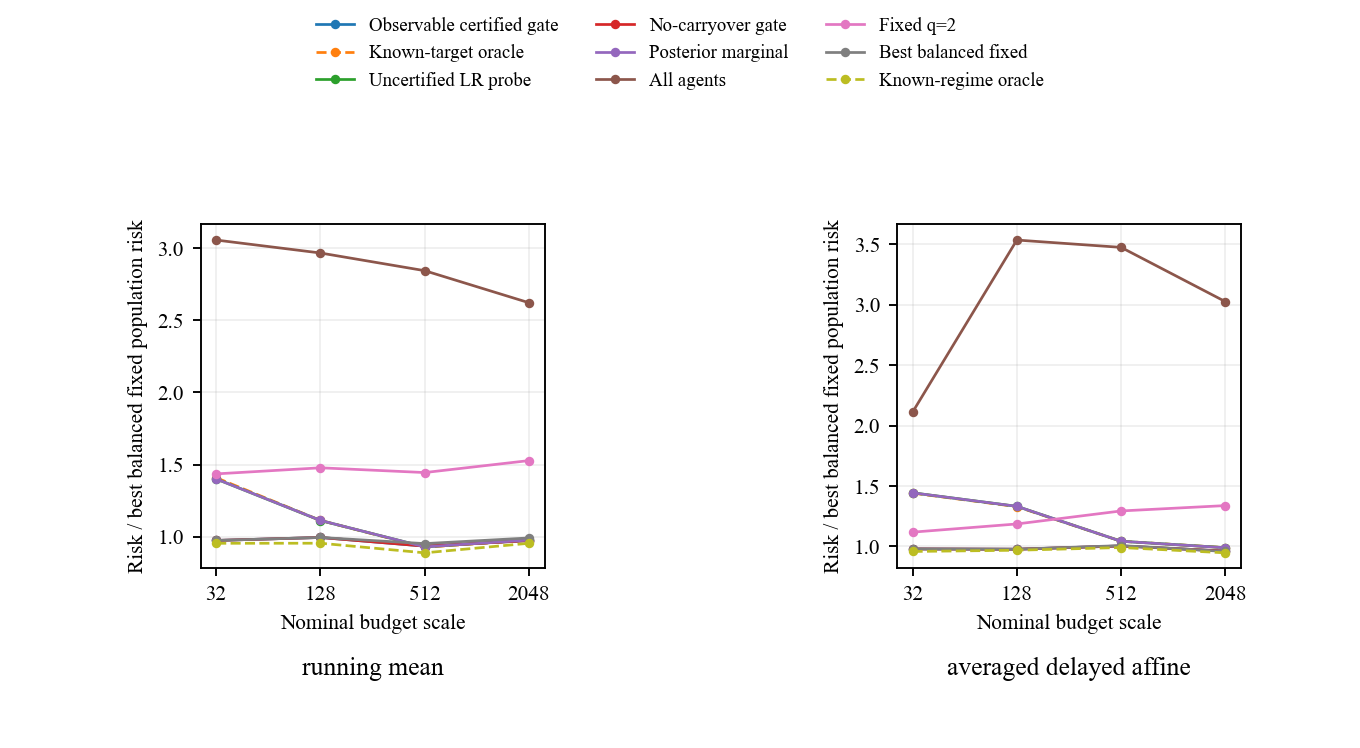
\includegraphics[width=\textwidth]{figures/observable_learner_budget_20261021.png}
\caption{Observable study using the larger empirical mean over the two fixed hidden signs for each learner and budget. This descriptive maximum is not a uniform confidence guarantee.}
\label{fig:observable-sign}
\end{figure*}
